%{\let\newpage\relax\maketitle}

%\iffalse
%\newpage
\clearpage
%\thispagestyle{plain}
\thispagestyle{empty}
\vspace*{3.8cm}
%\begin{center}
%    \emph{For the love of Science}
%\emph{``Equipped with his five senses, man explores the universe around him and calls the adventure Science.''} --- Edwin Hubble, 1929
\hspace*{0.5cm}\begin{minipage}[c]{0.5\linewidth}
\epigraph{``\emph{Equipped with his five senses, man explores the universe around him and calls \phantom{``}the adventure Science.}''}{--- Edwin Hubble, 1929}
\end{minipage}
\vspace*{3cm}%{6cm}
\begin{center}
\begin{minipage}[c]{0.66\linewidth}%
\begin{center}%
%\fbox{%
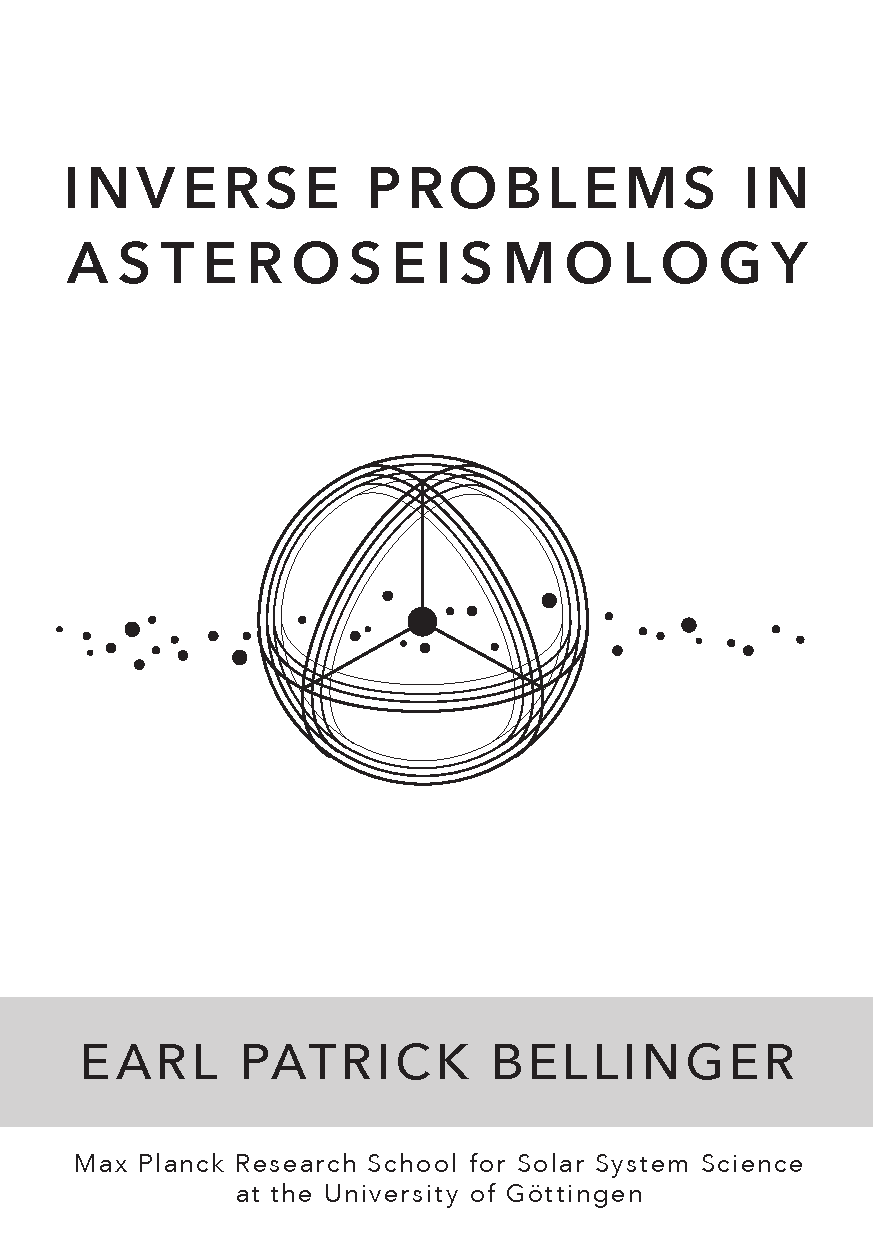
\includegraphics[width=\linewidth,trim={1cm 7cm 1.55cm 7cm},clip]{thesis_logo.pdf}%
%}%
\end{center}
\end{minipage}
\end{center}
%\vfill
\vspace*{0.5cm}
\noindent{\normalsize\bfseries\scshape\sffamily{About the Cover.}} An artist's depiction of a star's interior being revealed through its oscillations. 
The background shows stars from the constellation of Cygnus, which was observed for four continuous years by the \emph{Kepler} space observatory. 
The cover was created for use in this thesis by \href{http://kcaseyshea.com/}{K.\ Casey Shea}.
%\end{center}
%\newpage
%\clearpage
%\fi
%\clearpage
%\newpage
%\newpage
\clearpage